\chapter{State of the Art}
%What was given to me
In this chapter informations about the current project are revealed. At the beginning the properties of the project are explained and later in this chapter the simulation program is presented. The sections \ref{sec:Adhesion} to \ref{sec:3D} are explained based on the program of the project, whereas the other sections are presented based on previous work of the project.

\section{Moduro}
In the project moduro stands for 'Modeling of the Urothelium with the \ac{GGH} approach'. The department of Medical Informatics at the University of Applied Sciences Mannheim and the Clinic of Urology in cooperation with the Medical Faculty Mannheim at the University of Heidelberg participate in this project. The aim is to predict how and when bladder cancer arises.

The current moduro project has a stable 2D simulation of 16 different models. The simulations are performed by \ac{CC3D}. During the simulation statistics about the current simulation are written in text files and can be read out by the moduro toolbox. \newline
The project consists of a program and several models, both are written in Python. The models include properties of cell behavior. Therefore, the adhesion energy between cells and the possibilities of the new cell types after mitosis are defined in the different models. The application modifies the cell behavior, for instance it checks when a mitosis takes place and how fast the cell will grow.


\section{Display and simulation of the urothelium}
%wie wird es dargestellt 
In the 2D simulation, the urothel is simulated with a size of \SI{500}{\micro\metre} for the x-axis and \SI{150}{\micro\metre} for the y-axis. Since the voxel density is $0.8$, the size of the urothelium is represented by 400 pixels at the x-axis and 120 pixels at the y-axis. The voxel density describes how many pixels are used to display \SI{1}{\micro\metre}. \ac{CC3D} allows the user to use any simulation size, as long as the required hardware is able to handle the simulation. \newline
It is possible to use \ac{CC3D} on several cores of the CPU. In the project one core for a simulation is used, because otherwise \ac{CC3D} splits the simulation field into different grids. As a result race conditions can occur at the edges of these grids \cite{MaciejH.Swat2017}. This means it is possible that a cell is in two grids, one half is in one grid and the other half is in another grid. During the simulation both grids would calculate the volume of the cell and both would apply the new volume of their calculation, but it is not checked which result has to be used. Therefore, in order to reduce wrong results, it is necessary to avoid race conditions. \newline 
The 2D simulations of the urothelium cover a timespan of 720 days. In the simulations one day is split up into 500 \ac{MCS}. Therefore, the simulation covers 360000 \ac{MCS}. The simulation duration can be set in the program. The user defines how many \ac{MCS} simulate one day and how long the simulation runs. At the first calculation step, \ac{MCS} 0, the simulation is initialized. An illustration of an initial simulation is displayed in figure \ref{img:2DSimulationInitialState}. The urothelium is proposed to grow and to proliferate in the given area, because morphogenesis is simulated. An illustration therefor is presented in figure \ref{img:2DSimulation33Days}.


\begin{figure}[ht]
	\center
	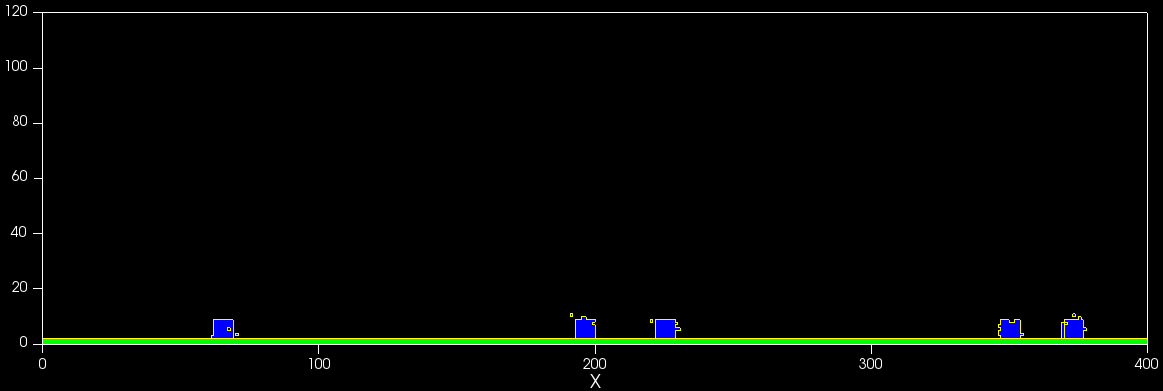
\includegraphics[scale=0.35]{figures/2DSimulation-InitialState.png}
	\caption{Initial state of a 2D simulation of the model SPA/BPCD/IPCD.}
	\label{img:2DSimulationInitialState}
\end{figure}

\begin{figure}[ht]
	\center
	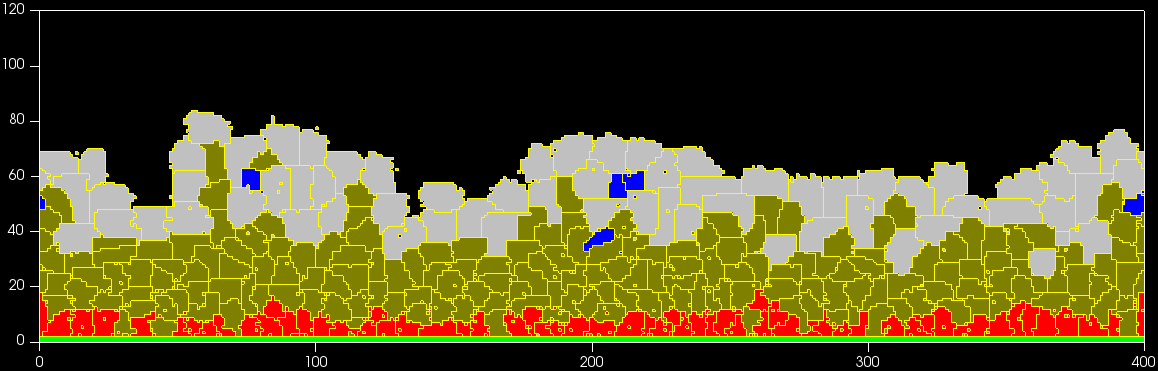
\includegraphics[scale=0.35]{figures/2DSimulation-33Days.png}
	\caption[2D Simulation of the model SPA/BPCD/IPCD after 33 days]{2D Simulation of the model SPA/BPCD/IPCD after 33 days. This figure displays a chaotically urothel, as the stem cells (the blue cells) are not at the basal membrane.}
	\label{img:2DSimulation33Days}
\end{figure}

\section{Moduro toolbox}
The moduro toolbox is a software tool, which visualizes data in order to evaluate a simulation. \newline
Every twelve hours the simulation is checked for its reality. This is done with the fitness functions of section \ref{sec:fitnessFunctions}. The results of these calculations are written in several text files in a by \ac{CC3D} created directory. The amount of cells of the different cell types and the overall amount of cells is saved as well. The moduro toolbox is able to read out the data of the text files and then visualize these. This visualization is done with charts and with a table. \newline
\ac{CC3D} saves some screenshots of the simulation field during the simulation. With these screenshots the moduro toolbox is able to create a video out of these screenshots. To create the video an extra program has to be installed which the toolbox  uses.

\section{Proliferation models}\label{sec:Models}
The 2D simulation of the urothel provides 16 different models. These models differ in which cell types after the mitosis are created. \newline 
At the initialization of a simulation stem cells are created and drawn on the basal membrane. These stem cells grow and split into basal cells. The basal cells grow and split into intermediate cells. These intermediate cells grow and split into umbrella cells. Therefore, for every proliferation model of the stem cells every model of the basal cells is used and for every model of the basal cells every model of the intermediate cells is used. \newline
With these mitosis concepts there are 16 different models in the project. These models were created by an earlier version of the project \cite{Torelli2017} and are displayed and summarized in table \ref{tbl:16Models} at page \pageref{tbl:16Models}. The different proliferation concepts are explained in the following subsections.

\subsection{Stem cells}
The stem cells are the first type of cells which undergo mitosis. One concept has the identifier 'SSD' and the other one is called 'SPA'. In the first model it is modeled that every time a stem cell divides there will be one stem and one basal cell. In the second model the stem cell has a probability of 90\% that it will be one stem and one basal cell after mitosis. There is also the chance with a probability of 5\% each that after mitosis of a stem cell there are two stem cells or two basal cells.
\subsection{Basal cells}
For the mitosis of basal cells there are 4 different models. The mitosis model 'BSD' describes that each basal cell which undergoes mitosis will create one basal and one intermediate cell. The model 'BPA' describes that there is either a 5\% chance that the basal cell will become two basal or two intermediate cells. There is a 90\% probability that the cell become one basal and one intermediate cell. The model 'BPCD' describes that always a basal cell becomes two basal cells during mitosis and if the basal cell is not on the basal membrane it transforms into an intermediate cell. The model 'BCD' has the behavior that a basal cell immediately transforms into an intermediate cell if it is not at the basal membrane.\newline
\subsection{Intermediate cells}
There are two different models how intermediate cells split. One is the 'IPCD' where during mitosis an intermediate cell becomes two intermediate cells. Each \ac{MCS} it is checked if there is a cell around the intermediate cell. If this is not the case it is transformed into an umbrella cell. The second model is the 'ICD'. In this concept, the transformation of intermediate cells into the umbrella cells only happens if the intermediate cell is not enclosed by other cells. \newline


\section{Adhesion}\label{sec:Adhesion}
During morphogenesis the cells not only grow, they arrange themselves as well. For cell sorting there have to be different adhesion values, i.e. how strong two different cells are holding on to each other. In the project this is done with a matrix, which is applied for every one of the 16 models. Such a matrix was created in an earlier version of the project \cite{Torelli2017} and is displayed in table \ref{tbl:AdhesionMatrix} at page \pageref{tbl:AdhesionMatrix}.


\section{Cell properties}
In the project the physiological constraints of a cell are included. In an earlier version of the project these were evidenced \cite{Torelli2017} and are displayed in table \ref{tbl:CellConstraints} at page \pageref{tbl:CellConstraints}. In the program these constraints are converted into pixels and then applied. \newline
In the simulation every cell has several attributes. Moreover, each cell has a cell dictionary in which additional attributes are stored. The properties regarding the cell type are likely what every cell in general has, e.g. a min-max diameter, a min-max volume, growth in \SI{}{\micro\metre} per day or the time until apoptosis, i.e. cell death. \newline
The attributes in the cell dictionary are mainly used for decision making. Some values are the current and expected live time, a flag for necrosis and if a cell is inhibited, i.e. enclosed by other cells. \newline


\section{Events in the simulation}
In the simulation program there are several events modeled. These events can occur at every calculation step or at a specific \ac{MCS} in the simulation. \newline
The events which are performed every \ac{MCS}, except for \ac{MCS} 0 and every \ac{MCS} of factor 250, are a) cell growth, b) the check for mitosis, c) cell death, d) cell transformation and e) cell mutation. The event which occurs every twelve hours, every 250 \ac{MCS}, is f) urination. These events are presented in detail in the following subsections.

\subsection{Cell Growth}
In the project the maximum possible growth of a cell is calculated and applied. This calculation is used for the relation volume and target volume as well as for the relation volume, surface and target surface. Because the volume and the surface of a cell are calculated by \ac{CC3D} and can only be read out, the target volume and target surface are calculated in the program and set.

\subsection{Mitosis}
The verification when a cell divides or grows further is done in every simulation step, except for these with a factor of 250. Therefore, it is possible to define a very specific calculation step at which a cell divides, as there are 500 \ac{MCS} per day. In order that a cell divides it grows over its maximal size before it divides.
The cells which are able to grow and as a result divide are a) stem cells b) basal cells and c) intermediate cells. The umbrella cells grow as well, but they do not split.

\subsection{Necrosis}
If a cell dies, necrosis takes place. In the program a flag in the cell dictionary is set. Every calculation step, the program checks if a cell dies or not. If so, the cell will shrink and as a result disappear.

\subsection{Mutation}
After two days, 1000 \ac{MCS}, it is possible that a cell mutates, i.e. it becomes malignant. Each cell type has its own probability to become malignant. In the current simulation it is not considered that cells mutate since the probability for each cell type to mutate is 0\% in the program. \newline
If a cell mutates, there is also the flag for necrosis set. Thus, the cell shrinks and disappears.

\subsection{Transformation}
A transformation can take place if at least one intermediate cell is created. If the intermediate cell is not enclosed by other cells, it is transformed to an umbrella cell.

\subsection{Urination}
Every twelve hours, every 500 \ac{MCS}, a urination takes place. The first urination event takes place at \ac{MCS} 375. This is simulated in a way that randomly 2\% of the cells in direct contact with the bladder are washed out. In the program a flag for necrosis is set and the cells will disappear because of the necrosis event.



\section{Fitness functions}\label{sec:fitnessFunctions}
In order to validate the simulated models, there are several functionalities which check if the model is realistic or not. These functions check every twelve hours, every 250 \ac{MCS}, if the model is realistic or not. The results of these fitness functions are written into several files and can be read out by the moduro toolbox.

\subsection{Arrangement fitness function} \label{subsec:ArrangementFitness}
The arrangement fitness function ensures that the strata of the simulated urothelium has the correct order \cite{Torelli2017}, i.e. that the first layer on the basal membrane consists only of stem and basal cells \cite{Yamany2014, Lazzeri2006}, the next three to five layers consist only of intermediate cells \cite{PuneetKhandelwal2009} and that there is one layer of umbrella cells \cite{PuneetKhandelwal2009, Yamany2014}.

\begin{equation}\label{eq:LIB}
lib = \dfrac{L - lib}{L}
\end{equation}
\begin{equation}\label{eq:FitnessArrangement} 
f_{A} = 1 - \dfrac{((1-L_{B})+(1-L_{U})+lib+(1-L_{O})}{4}
\end{equation}
In equation \ref{eq:LIB} $L$ refers to the amount of layers in the urothelium. $lib$ describes the amount of layers between the stem and basal cell layer and the umbrella cell layer at the top of the urothelium, which includes not only intermediate cells. Thus, if the layers between the first and last layer consist only of intermediate cells the equation \ref{eq:LIB} has the result 0.\newline
In equation \ref{eq:FitnessArrangement} $L_{B}$ and $L_{U}$ are boolean values, i.e. they have the value zero or one and represent a false or true value. They are one if the first layer of cells consists only of basal or stem cells and if the most upper layer consists only of umbrella cells, otherwise they will be zero.
$lib$ is calculated in equation \ref{eq:LIB}. $L_{O}$ presents the optimum amount of layers. It is one, if the amount of layers in the simulated urothelium is between three and seven, otherwise it is zero. The result of equation \ref{eq:FitnessArrangement} is between zero and one, where zero refers to a chaotically grown urothel with an unrealistic structure and one refers to a perfectly structured urothelium. \newline

\subsection{Volume fitness function} \label{subsec:VolumeFitness}
This function calculates the relative volume regarding the current volume of the different cell types in the urothel. The relative amount of the different cell types should be: stem and basal cells = 10\%, intermediate cells = 67\% and umbrella cells = 23\% considering an average thickness of \SI{85}{\micro\metre} \cite{Torelli2017}. Therefor the formula is:
\begin{equation}\label{eq:VolumeFitnessSpecific}
f_{V_{i}} = \dfrac{1}{4 (\dfrac{V_{Si}-V_{Ii}}{V_{Si}})^2 + 1}
\end{equation}
$V_{Si}$ and $V_{Ii}$ describe the should (target) and the actual is (current) volume of a specific cell type $i$ \cite{Torelli2017}.  This calculation is done three times. One time for the stem and basal cells, one time for the intermediate cells and one time for the umbrella cells. The results of the three calculations are then further used to determine the relative volume overall.
\begin{equation}\label{eq:VolumeFitnessOverall}
f_{V} = \dfrac{f_{V_{B}} + f_{V_{I}} + f_{V_{U}}}{3}
\end{equation}
In equation \ref{eq:VolumeFitnessOverall} $f_{V_{B}}$ refers to the relative volume of the stem and basal cells, $f_{V_{I}}$ presents the relative volume of the intermediate cells and $f_{V_{U}}$ includes the relative volume of the umbrella cells. \newline
The result of all four calculations, three times the equation \ref{eq:VolumeFitnessSpecific} for every layer and one time equation \ref{eq:VolumeFitnessOverall} is calculated and written into a text file and can be read out by the moduro toolbox later.


\subsection{Overall fitness function}
The ideas and equations presented in the following subsections are found in the paper created earlier in the project \cite{Torelli2017}. In the program this functionality is only in the class 'OptimumSearchSteppable'. This functionality was commented out and therefore it was not used in the program. \newline
The overall fitness function calculates the total fitness out of the volume and the arrangement fitness function. Therefore, the average of both functions is calculated. For every calculation step, the arrangement and volume fitness function are calculated and the overall fitness is calculated. Therefore, the formula is:

\begin{equation} 
f(t_{i}) = \dfrac{f_{V}(t_{i})+f_{A}(t_{i})}{2}
\end{equation}

$t_{i}$ describes a specific point of time, in \ac{MCS}, at which this calculation is done. At the end of the simulation the average of the overall fitness function is calculated to determine the reality of this simulation. Therefore, the formula is:
\begin{equation} 
f = \dfrac{1}{e+1} + \sum_{i=0}^{e}{f(t_{i})}
\end{equation}
The result of the calculation is between zero and one, where zero describes no reality at all and one presents a perfect realistically simulated urothelium.


\section{3D functionalities }\label{sec:3D}
The functionalities of the program are able to be used in 3D. Whenever a part of the program is required to be used in 2D as well as in 3D it is checked if the simulation field has a third dimension or not. Examples for such functionalities are the fitness functions of the section before or the decision how many stem cells are placed on the basal membrane, which is modified and explained in section \ref{sec:AmountStemCellsBasalMembrane}. \newline
It is important to keep the functionalities of the 2D simulation in the program, because so far only the 2D simulations were progressed. Doing so it is possible to switch between a 3D and a 2D simulation. Thus, the benefits of both simulation types can be observed.


\begin{table}[ht]
\begin{centering}
\caption[Adhesion matrix, which was used earlier in the project]{\label{tbl:AdhesionMatrix}Adhesion matrix for a model in the simulation. Smaller values refer to more adhesion and higher values mean less adhesion. The cell type M is the medium cell type, it is by \ac{CC3D} a specific cell type which is everywhere in the available space in the simulation, and BM is the basal membrane. This table was created in an earlier version of the project \cite{Torelli2017}. \newline}
\begin{tabular}{|c|c||c|c|c|c|c|c|}
\hline 
\multicolumn{2}{|c||}{Types} & M & BM & \celltypeS & \celltypeB & \celltypeI & \celltypeU \tabularnewline
\hline 
\hline 
Medium & M & 0 & 14 & 14 & 14 & 14 & 4\tabularnewline
\hline 
Basal membrane & BM &  & -1 & 1 & 3 & 12 & 12\tabularnewline
\hline 
Stem cell & \celltypeS &  &  & 6 & 4 & 8 & 14\tabularnewline
\hline 
Basal cell & \celltypeB &  &  &  & 5 & 8 & 12\tabularnewline
\hline 
Intermediate cell & \celltypeI &  &  &  &  & 6 & 4\tabularnewline
\hline 
Umbrella cell & \celltypeU &  &  &  &  &  & 2\tabularnewline
\hline 
\end{tabular}
\par\end{centering}
\end{table}



\begin{table}[ht]
\begin{centering}
\caption[Constraints of the different cell types]{\label{tbl:CellConstraints}Constraints of the different cell types. Volumes $V$ in $\mu$m$^{3}$, diameters $d$ in $\mu$m. The 'Volume' and 'Surface' column describe how the $\lambda_{vol}$ and the $\lambda_{sur}$ should be set for each cell type. This table was created in an earlier version of the project \cite{Torelli2017}. \newline}
\begin{tabular}{|cc|c|c|c|c|c|c|}
\hline 
Cell type & & $V_{min}$ & $d_{min}$ & $V_{max}$ & $d_{max}$ & Volume & Surface\tabularnewline
\hline 
\hline 
Stem & \celltypeS & 268 & 8 & 523 & 10 & perfect & average\tabularnewline
\hline 
Basal & \celltypeB & 381 & 9 & 523 & 10 & important & average\tabularnewline
\hline 
Intermediate & \celltypeI & 905 & 12 & 1767 & 15 & important & poor\tabularnewline
\hline 
Umbrella & \celltypeU & 1767 & 15 & 3591 & 19 & important & poor\tabularnewline
\hline 
\end{tabular}
\par\end{centering}
\end{table}




\begin{table}[ht]
\begin{centering}
\par\end{centering}
\begin{centering}
\caption[16 different models in the project]{\label{tbl:16Models}16 different models derived from an earlier version of the project \cite{Torelli2017} as there are different ways of proliferation and mitosis beeing simulated for the different cell types. S refers to the stem cell wheras B displays a basal cell. I presents the intermediate cell and U refers to the umbrella cell. BM displays the basal membrane and M presents the Medium cell type, which is a by \ac{CC3D} specific cell type. \newline}
\begin{tabularx}{\textwidth}{|c|c|Xc|}
\hline 
Type & ID & Description & Model\tabularnewline
\hline 
\hline 
\multirow{2}{0.02\textwidth}{\begin{turn}{90}
Stem cells
\end{turn}} & SSD & Stem cell-like division & \begin{tikzpicture}[]
\node[SType] {S} [grow=right]
	child {node [SType]  {S}
	}
	child {node [BType]  {B}
	};
\end{tikzpicture}\tabularnewline
\cline{2-4} 
 & SPA & Stem cell population asymmetry & \begin{tikzpicture}[]
\node[SType] {S} [grow=right]
	child {node [SType]  {S}
	}
	child {node [SType]  {S}
	};
\node at (0.5,-1) {$p_s=0.05$};
\node[SType] at (2,0) {S} [grow=right]
	child {node [SType]  {S}
	}
	child {node [BType]  {B}
	};    
\node at (2.5,-1) {$p_a=0.90$};    
\node[SType] at (4,0) {S} [grow=right]
	child {node [BType]  {B}
	}
	child {node [BType]  {B}
	};    
\node at (4.5,-1) {$p_s=0.05$};        
\end{tikzpicture}
\tabularnewline
\hline 
\multirow{4}{0.02\textwidth}{\begin{turn}{90}
Basal cells\ \ \ \ \ \ \ \ \ \ \ \ \ \ \ \ \ \ \ \
\end{turn}} & BSD & Stem cell-like division in basal cell & 
\begin{tikzpicture}[]
\node[BType] {B} [grow=right]
	child {node [IType]  {I}
	}
	child {node [BType]  {B}
	};
\end{tikzpicture}
\tabularnewline
\cline{2-4} 
 & BPA & Basal cell population asymmetry & \begin{tikzpicture}[]
\node[BType] {B} [grow=right]
	child {node [BType]  {B}
	}
	child {node [BType]  {B}
	};
\node at (0.5,-1) {$p_s=0.05$};
\node[BType] at (2,0) {B} [grow=right]
	child {node [BType]  {B}
	}
	child {node [IType]  {I}
	};    
\node at (2.5,-1) {$p_a=0.90$};    
\node[BType] at (4,0) {B} [grow=right]
	child {node [IType]  {I}
	}
	child {node [IType]  {I}
	};    
\node at (4.5,-1) {$p_s=0.05$};        
\end{tikzpicture}\tabularnewline
\cline{2-4} 
 & BPCD & Proliferation and contact differentiation of basal cells & \begin{tikzpicture}[]
\node[BType] {B} [grow=right]
	child {node [BType]  {B}
	}
	child {node [BType]  {B}
	};
\end{tikzpicture} \hspace{1em} and \hspace{1em}
\begin{tikzpicture}[]
\node[BType] {B} [grow=right]
	child[dashed] {node [IType] {I} edge from parent node[above=0.4cm] {$\neg$ BM}
	};
\end{tikzpicture}\tabularnewline
\cline{2-4} 
 & BCD & Only contact differentiation of basal cells & 
\begin{tikzpicture}[]
\node[BType] {B} [grow=right]
	child[dashed] {node [IType] {I} edge from parent node[above=0.4cm] {$\neg$ BM}
	};
\end{tikzpicture}\tabularnewline
\hline 
\multirow{2}{0.02\textwidth}{\begin{turn}{90}
Intermediate cells
\end{turn}} & IPCD & Proliferation and contact differentiation of intermediate cells & \begin{tikzpicture}[]
\node[IType] {I} [grow=right]
	child {node [IType]  {I}
	}
	child {node [IType]  {I}
	};
\end{tikzpicture} \hspace{1em} and \hspace{1em}
\begin{tikzpicture}[]
\node[IType] {I} [grow=right]
	child[dashed] {node [UType] {U} edge from parent node[above=0.4cm] {M}
	};
\end{tikzpicture}
\tabularnewline
\cline{2-4} 
 & ICD & Only contact differentiation of intermediate cells & 
\begin{tikzpicture}[]
\node[IType] {I} [grow=right]
	child[dashed] {node [UType] {U} edge from parent node[above=0.4cm] {M}
	};
\end{tikzpicture}
\tabularnewline
\hline 
\end{tabularx}
\par\end{centering}
\end{table}
